\documentclass[sigconf, 12pt]{acmart}
\begin{document}

\title{The Ethics of Generative AI in Commercial Software Development}
\author{Roman Marquez-Twisdale}
\email{r.marqueztwisdale@digipen.edu}

\date{Today}
\maketitle

\section{Introduction}
Over the past few years, generative AI has started to become a normal part of software development. Models capable of generating code from simple prompts are now used by students, developers, and large companies working on commercial software. In some ways this seems like a huge benefit. Developers can work more efficiently in a lot of cases. ~\cite{(11)} Due to this, it’s not surprising that many software companies would start to partially rely on AI-generated code in the development of their real-world applications. But just because something is useful doesn’t make it ethical, especially if that code is being shipped in commercial products.
\subsubsection{Irresponsible Development}
One of the biggest issues is how it’s being used. In many cases, developers might not fully understand the code that the AI produces, yet still include it in finished products. This makes is more likely that something will break or introduces a security issue. There’s also the problem of transparency. If developers don’t acknowledge when or how AI was used, how do we know who wrote a piece of software? How do we know who owns a piece of software? These problems are only amplified in commercial settings, where software affects real users.
\subsubsection{Copyright Issues}
There are larger concerns about where AI-generated code comes from. Since these systems are trained on large amounts of existing code, much of which was scraped from the internet, including open-source projects, they might reproduce patterns or structures without proper acknowledgement to the original authors.
\subsubsection{Core Argument}
This paper argues that using machine learning models to generate code for commercial applications is only ethical under certain conditions. Specifically, developers need to understand the code they use and be transparent about how AI contributed to the final product.


\section{Background}
To understand the ethical issues around AI-generated code in commercial software, lets clarify what is being discussed and who is affected. Software engineers range from individual developers working on small projects to large teams building complex systems. Generative AI refers to Large Language Models that produce code from natural language prompts, often trained on massive datasets containing publicly available code and documentation. Commercial applications includes software sold on the open market, and internal systems which play any role in the development of the software being sold.
The ethical concern arises because LLMs are not currently held responsible for the code they generate and neither is their creators. The generated code is not fully written by the developer and not clearly belonging to any single original source.
\subsubsection{Highlights}
Research has shown that generative AI systems can reproduce patterns from training data. "According to the award-winning website Copyleaks, nearly 60\% of the responses provided by Defendants’ GPT-3.5 product in a study conducted by Copyleaks contained some form of plagiarized content, and over 45\% contained text that was identical to pre-existing content." ~\cite{(7)} These models are also known to produce inaccurate or misleading outputs, sometimes referred to as “hallucinations,” which can make their use risky in real-world applications. ~\cite{(3)}


\section{Stakeholders}
Software engineers benefit from increased productivity but if not careful, can end up with software they don't fully understand.
Companies gain efficiency but weaken their legal and ethical security, especially if AI-generated code includes copyrighted material without. "researchers warn that black-box AI tools may blend code from multiple sources, risking inadvertent violations." ~\cite{(9)}
End users are also affected, even if indirectly. They depend on software to function as intended, bugs and vulnerabilities impact them directly. AI-generated content has already been seen in other domains, creating challenges for maintaining quality and trust in all communities. "It’s unlikely that any human editor or technology can sustain an ability to differentiate human from machine writing." ~\cite{(10)}
The open-source community is another important stakeholder. Many AI systems are trained on publicly available software, often without explicit consent from contributors. This raises concerns about respect for intellectual labor. ~\cite{(7)}
Finally, the organizations that develop AI systems also play a role. These organizations are at the forefront of ethical guidelines adoption. If they choose to emphasize transparency, and accountability, they could have a powerful impact on the emerging technology, but this may come at a cost. ~\cite{(4)} ~\cite{(8)}

\section{Current State of Generative AI}
Many developers now use LLMs for tasks like writing basic code, debugging, and documentation. Developers can generate functional code much faster than writing everything by hand. Research suggests these tools are particularly effective for documentation, testing, and basic implementation. ~\cite{(6)}
However, these benefits come with a cost. AI-generated code is not always correct and can contain logical errors or subtle bugs. Even when it appears correct, it may include poor design choices. Security is another concern. Research has found that AI-generated code can include unsafe practices, and many developers do not consistently review it before use. ~\cite{(6)} 
There is also the issue of over-confidence. Developers might use AI outputs without fully checking them, even if they don’t completely trust them. Over time, this can also affect skill development, as developers rely more on AI instead of problem-solving themselves. ~\cite{(6)}
Overall, generative AI is powerful but potentially dangerous. It works well for simple tasks but struggles with more complex problems, making human oversight essential for responsible development.


\section{Technical Background}
To understand why AI-generated code can be risky, it helps to have a basic idea of how these models work. Most modern generative AI tools are based on large language models, which are trained on massive datasets. During training, the model learns patterns in how words and code are structured, but it is commonly believed that it doesn't actually “understand” what it is generating in a human sense. ~\cite{(6)}

\subsubsection{High Level}
These models work by breaking input text into smaller pieces called tokens and then predicting what token should come next based on a learned pattern. When a developer submits a prompt to a Large Language Model, the model processes it and generates code one token at a time using a Recurrent Neural Network (RNN), a type of neural network that feeds it's own outputs back into itself in order to remember and use previous states to help predict future states. "While the ‘meaning’ of these tokens is implicit to some extent within these associations, the model is not explicitly utilising this meaning, but is rather generating syntactically appropriate strings of text based on statistical associations." ~\cite{(3)}

\begin{figure}[h]
  \centering
  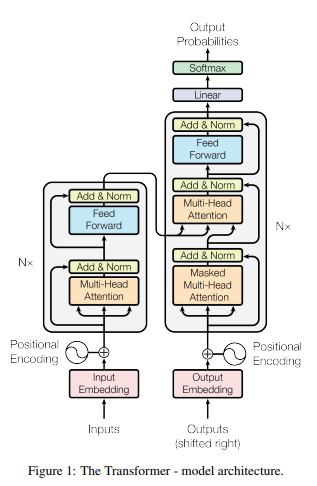
\includegraphics[width=\linewidth]{EncoderArchitecture}
  \caption{The Encoder-Decoder Transformer Architecture.}
  \Description{A graph of neural network.}
\end{figure}
 
One of the most common LLMs used today is ChatGPT. The acronym "GPT" stands for Generative Pre-Trained Transformer and represents one of the most common architectures used today. In 2017, the paper "Attention Is All You Need" was published describing this architecture.

\subsubsection{Encoder}
Within this model architecture, the inputs are encoded into value sequences and passed through a section of the network known as the Multi-Head Attention mechanism. They are then passed through a traditional feed forward neural network. After each of these steps there is a normalization process. Finally, the encoder produces an encodes sequence of values that can be passed through the decoder to produce the final result.

\subsubsection{Decoder}
The Decoder is fed all previous outputs along with the current encoded input. Both the previous outputs and the encoded input are passed through their own Multi-Head Attention mechanisms, and then combined to produce a final result for the next token in the sequence. It is the previous tokens which allow for this architecture to recognize patterns and adjust its behavior based on what came before. If we didn't pass in the previous token outputs during the computation of each subsequent token, we would essentially be stripping the model of any long term memory. very likely, the model wouldn't be able to produce text longer than a few sentences.

\subsubsection{Attention}
The Multi-Head Attention blocks within this structure maps a query and set of key-value pairs to an output. The output is computed as a weighted sum of the inputs. the queries, keys and values are all represented as vectors.

\begin{figure}[h]
  \centering
  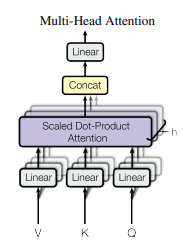
\includegraphics[width=\linewidth]{Attention}
  \caption{The Encoder-Decoder Transformer Architecture.}
  \Description{A graph of neural network.}
\end{figure}

These transformers uses multi-head attention in three ways. The encoder-decoder attention layers source the queries from the previous decoder layer. The memory keys and values come from the output of the encoder. "This allows every position in the decoder to attend over all positions in the input sequence." ~\cite{(2)} The encoder makes use of self-attention layers. In a self-attention layer all the keys, values and queries come from the output of the previous layer's encoder. "Each position in the encoder can attend to all positions in the previous layer of the encoder." ~\cite{(2)} Similarly, self-attention layers in the decoder allow each position to attend to all previous positions including the current position within the sequence.

As fancy as these systems are, they remain a black box to all humans, even those who understand them best. 




\section{Ethical Analysis}
Social Contract Theory provides a useful framework for evaluating these issues. It is based on the idea that society functions through shared expectations and beliefs. Honesty, fairness, and accountability are by no means enforced by mother nature, but are valued by most who would like to live in a society.
\subsubsection{Software Development Contract}
In software development, there is an implicit agreement that developers understand and take responsibility for the code they write. When developers rely on machine learning models to generate code without fully understanding it, this weakens trust. If something goes wrong, responsibility becomes unclear, which violates the expectation that developers stand behind their work. Transparency is another key part of this social contract. If developers do not acknowledge the use of AI in their code and present their work as entirely their own, this raises concerns about fairness and authorship. This is important given that these models are trained on other developers contributions. ~\cite{(7)}
\subsubsection{Open Source}
There is also an implicit agreement with the open-source community. Engineers share their work expecting due credit, but AI systems may produce similar code without referencing the original author's work they were trained on. Social Contract Theory does not imply that the use of these models is always unethical. If developers review and understand the code they use, and if commercial organizations are transparent about how models were or were not used in their products and services, they can reap the benefits of such tools without uprooting societies expectations for ethical software development.

\section{Safeguards and Responsibilities}
Given the current state of generative AI, the main issue is how it is used. Making AI-generated code ethical comes down to policy. One of the most important safeguards we can implement is requiring developers to thoroughly review and understand any AI-generated code before using it commercially. AI can produce incorrect or misleading outputs. As such, blindly trusting it can lead to bugs and security issues. ~\cite{(3)} ~\cite{(5)} Transparency must be considered as well. Software developers and companies should acknowledge when machine learning models are used in commercial projects. Without this, it becomes harder to assign responsibility or identify sources. ~\cite{(8)} And as soon as the standards such as requiring code reviews and training developers on risks become widely known, it will be the responsibility of companies to enforce these standards. Last but not least, the organizations that develop these models share responsibility for how they are trained, how data is acquired, and what data is used.

\section{Conclusion}
Generative AI offers clear benefits in terms of productivity and accessibility, but that does not mean its use is ethical. The main concerns are lack of understanding and lack of transparency. When developers use AI-generated code without fully understanding it, they take responsibility for something they did not create entirely on their own. When they fail to acknowledge AI use, it breaks social contracts around honesty and ownership. From an ethical perspective, developers still have a responsibility to ensure their code is correct and safe, regardless of how it was created. Even more importantly, misuse of these models can reduce trust in software systems and the development pipelines they came from, creating unfair conditions for others. ~\cite{(8)} Developers need to understand and verify the code they use, companies need clear generative AI policies, and there needs to be transparency about how machine learning models are used in commercial settings. Without these safeguards, the risks can outweigh the benefits. I think about using AI tools in my own work. It’s easy to rely on them for quick answers, but that doesn't mean I actually understand what I’m building. Going forward, I think the most important takeaway is that using AI responsibly means treating it as a tool, not a replacement for critical thinking. If developers can do this, these kinds of models can be a helpful part of the development process. If not, they introduce shortcuts that creates more problems than they solve.

\section{Beyond the Superficial}
As an entry-level engineer entering the industry, I have no idea what my skills will be used for. I could end up working a job where I actually write code by hand, but that seem less common nowadays. The high likelihood that I will be generating code though some kind of machine learning model and then testing it means I need to start thinking about what kinds of responsibilities I will have when the time comes. It has always been hard for me to feel good about something I've done, if I lied about some portion of it. So I'm not too worried about myself using AI irresponsibly. What I am worried about is three fold.
\subsubsection{Global Impacts}
What kind of impact does this new technology have on the planet. Humans are not the only form of life trying to exist. Personally, I would rather live in a world with other life forms.
\subsubsection{Ethical Creation}
Are the manufacturers of such models being ethical in their creation of their models? Is their training data ethically sourced? Are their models bias?
\subsubsection{Maintaining Sanity}
And finally, do I have the ability to detect the use of AI in other works of art or engineering. If one day it becomes impossible to know what was created by humans because AI-generated content is indistinguishable, I personally will feel very uncomfortable. This kind of future is likely, and I'd imagine similar to the experience of an insane person. If we cannot tell what was created by a human, this is akin to being unable to tell what is real. Obviously there are differences, but the similarities are enough to make me care greatly about maintaining and supporting transparency when it comes to the use of AI-generated content.

\bibliography{bibliography}{}
\bibliographystyle{ACM-Reference-Format}
\end{document}